\documentclass[aps,prx,reprint,nofootinbib,longbibliography]{revtex4-2}

\usepackage[T1]{fontenc}
\usepackage[utf8]{inputenc}
\usepackage{amsmath}
\usepackage{amssymb}
\usepackage{bm}
\usepackage{booktabs}
\usepackage{graphicx}
\usepackage{hyperref}
\usepackage{xcolor}
\usepackage{listings}

\hypersetup{
  colorlinks=true,
  linkcolor=blue,
  citecolor=blue,
  urlcolor=blue
}

\lstdefinestyle{pegshield}{
  basicstyle=\ttfamily\small,
  breaklines=true,
  columns=fullflexible,
  frame=single,
  framerule=0.3pt,
  rulecolor=\color{black!35},
  xleftmargin=0pt,
  xrightmargin=0pt
}
\lstset{style=pegshield}
\graphicspath{{figures/}}

\newcommand{\bps}{\mathrm{bps}}
\newcommand{\clip}{\operatorname{clip}}
\newcommand{\E}{\mathbb{E}}
\newcommand{\Var}{\operatorname{Var}}
\newcommand{\dd}{\,\mathrm{d}}
\newcommand{\one}{\mathbf{1}}

\begin{document}

\title{PegShield: An On-Chain Risk Oracle Publishing\\Enforceable Collateral Constraints for\\Liquid-Staked Assets on Solana}

\author{Anubhav Prasai}
\affiliation{AI Youth Global Organization (AIYGO)}

\date{\today}

\begin{abstract}
Lending protocols govern liquid-staking-token (LST) collateral with static,
governance-set loan-to-value (LTV) factors that are revised on the timescale of
human risk review. During a de-pegging event, the borrow path moves faster than
governance can respond, and the same composability that makes an LST capital
efficient turns it into a correlated, illiquid collateral object. Price oracles
do not close this gap: they report what an asset is worth, not whether a lender
should keep extending credit against it. We present PegShield, a Solana-native
\emph{risk oracle} that publishes an enforceable lending constraint rather than a
price. Off-chain processes estimate peg-deviation dynamics from Pyth market prices
normalized by each token's canonical staking exchange rate, fit an
Ornstein--Uhlenbeck (OU) mean-reversion model, detect distress with a joint
Augmented Dickey--Fuller (ADF) and z-score regime rule, and apply bounded
liquidity and data-quality haircuts. The result is committed as a compact
fixed-point risk state---a suggested LTV in basis points plus a regime flag---to a
Solana program-derived address (PDA) that a lending market can read and enforce
directly inside its borrow logic. We formalize the published constraint as a
normalized solvency index $\Psi_t\in[\tfrac12,1]$, describe a bonded
threshold-attester update path with disputes and slashing that preserves the
consumer interface, and evaluate the system on a historical replay of the June
2022 stETH/ETH discount together with a battery of synthetic stress scenarios. In
the replay, the model emits its first protective signal before a fixed-80\% baseline
exhibits modeled shortfall; we report the resulting loss reduction as an upper bound
on the timing benefit rather than a causal guarantee. We are explicit about what this
evidence does and does not establish, and about the system's pre-production status. The contribution is a
concrete primitive: peg-deviation tail risk converted into a machine-readable,
on-chain credit boundary that downstream protocols can clamp, fall back from, or
use to halt new credit.
\end{abstract}

\maketitle

\section{Introduction}

Liquid staking resolves a capital-efficiency problem in proof-of-stake systems:
staked assets need not remain economically inert. On Solana, a high-throughput
proof-of-stake blockchain \cite{yakovenko2018solana}, receipt tokens such
as \texttt{mSOL}, \texttt{jitoSOL}, and \texttt{bSOL} represent claims on delegated
SOL and circulate through automated market makers, lending markets, and vaults
\cite{marinade_msol,jito_jitosol,solblaze_bsol}. Liquid staking is now one of the
largest categories of locked value in decentralized finance (DeFi)
\cite{defillama_lst}, and a substantial fraction of that value is pledged as
collateral in on-chain lending markets.

This composability produces a structural tension we call the
\emph{liquidity--staking paradox}: the same token that improves capital efficiency
under normal conditions becomes an unstable collateral object under stress. A
stake-pool receipt is redeemable against an underlying staking position, but
immediate secondary-market liquidity is finite and exit from the staking position
is subject to unbonding and withdrawal friction. When the receipt trades below its
canonical staking exchange rate, borrowers, liquidators, lenders, and arbitrageurs
may all demand exit liquidity in the same short interval. The June 2022
stETH/ETH discount on Ethereum---during which a liquid-staking receipt traded
persistently below parity with its underlying while leveraged holders
deleveraged---is the canonical illustration of how a liquid-staking peg can widen
faster than risk parameters are revised \cite{lido_steth_2022}.

The prevailing control for this risk is the collateral factor (equivalently, the
maximum LTV) set by protocol governance and periodically adjusted by risk
contributors \cite{aave2024docs,compound2019whitepaper,makerdao_whitepaper}.
Governance-set parameters are deliberate and auditable, but they are revised on a
human timescale---proposals, votes, timelocks---whereas a borrow transaction
executes in a single slot. Empirical studies of DeFi liquidations document how
quickly collateral quality can deteriorate and how liquidation activity clusters
in stress windows
\cite{qin2021empirical,perez2021knifeedge,gudgeon2020crisis,warmuz2022toxic}.
The mismatch between governance latency and borrow-path latency is precisely the
window in which new, undercollateralized credit is created.

Price oracles---Chainlink, Pyth, Uniswap time-weighted average prices (TWAPs),
and the Maker oracle security module---supply the value of collateral to these
markets \cite{breidenbach2021chainlink,pyth2022whitepaper,adams2021uniswapv3,makerdao_oracle_module}.
They are necessary but not sufficient for the problem above: a price feed answers
``what is this token worth?'' and is itself a documented manipulation surface
\cite{eskandari2021sok,zhou2023sok,daian2020flashboys,rekt_mango_2022}. It does
not answer the operational question a lender faces during a depeg: \emph{given
current peg deviation, estimated mean reversion, volatility, stationarity,
liquidity depth, and source quality, should this market extend new credit against
this collateral, and at what LTV?}

PegShield answers that question and commits the answer on-chain. It separates
price discovery from collateral-solvency control: a price oracle continues to
report value, while PegShield publishes a time-varying, enforceable lending
constraint keyed to a liquid-staking market. The answer lives in a Solana PDA, not
an off-chain dashboard, so a lending program can read the account, verify ownership
and freshness, and apply the suggested LTV (or a stricter local policy) inside its
own borrow path.

\paragraph{Contributions.}
This paper makes the following contributions.
\begin{enumerate}
\item \textbf{A risk-oracle primitive for LST collateral.} We define an on-chain
artifact whose output is an enforceable collateral constraint---a suggested LTV in
basis points and a regime flag---rather than a price, and we formalize it as a
normalized solvency index $\Psi_t\in[\tfrac12,1]$ (Section~\ref{sec:model}).
\item \textbf{A peg-deviation risk model.} We calibrate an Ornstein--Uhlenbeck
process to a peg-deviation signal that normalizes the market LST/SOL ratio by the
token's canonical staking exchange rate, and we classify distress with a joint
ADF/z-score regime rule, augmented by bounded liquidity and data-quality haircuts
(Sections~\ref{sec:arch}--\ref{sec:model}).
\item \textbf{An on-chain commitment and decentralized update path.} We describe a
compact fixed-point risk-state account and a bonded threshold-attester cycle with
disputes and slashing that decentralizes the writer while preserving a single,
stable consumer interface (Sections~\ref{sec:arch} and~\ref{sec:attester}).
\item \textbf{A reference enforcement model and an evaluation.} We give a
reference borrow gate that consumes the risk state, and we evaluate the system on a
historical stETH/ETH replay and a suite of synthetic stress scenarios, stating
precisely what the evidence supports (Sections~\ref{sec:consumer}--\ref{sec:eval}).
\end{enumerate}

The remainder of the paper reviews related work (Section~\ref{sec:related}),
describes the architecture (Section~\ref{sec:arch}) and statistical model
(Section~\ref{sec:model}), details the attester path (Section~\ref{sec:attester})
and consumer integration (Section~\ref{sec:consumer}), reports the evaluation
(Section~\ref{sec:eval}), analyzes security (Section~\ref{sec:security}), and
discusses limitations and threats to validity (Section~\ref{sec:discussion}).

\section{Background and Related Work}
\label{sec:related}

\subsection{Blockchain Oracles and Their Manipulation}

On-chain contracts cannot natively observe off-chain state, so oracles bridge
external data onto the chain \cite{beniiche2020study}. Chainlink aggregates reports from a decentralized
operator set \cite{breidenbach2021chainlink}; Pyth operates a first-party,
pull-based model in which publishers sign prices that consumers pull on demand,
each carrying a confidence interval \cite{pyth2022whitepaper,pyth_hermes}; Uniswap
v3 exposes a manipulation-resistant TWAP accumulator \cite{adams2021uniswapv3}; and
MakerDAO interposes an Oracle Security Module that delays price updates to bound
the impact of a compromised feed \cite{makerdao_oracle_module}. A complementary
design is the \emph{optimistic} oracle---most prominently UMA---in which a proposed
value is accepted unless disputed within a challenge window, with bonded
escalation to a vote \cite{uma_optimistic_oracle}.

Oracles are also a primary attack surface. Eskandari et al.\ provide a systematization
of oracle designs and the market-manipulation attacks they enable
\cite{eskandari2021sok}; broader systematizations of DeFi attacks catalogue
oracle-manipulation incidents as a dominant loss category
\cite{zhou2023sok}. Flash-loan-funded manipulation
\cite{qin2021flashloans,daian2020flashboys} and the October 2022 Mango Markets
exploit---in which an attacker inflated the price of thinly traded collateral to
borrow against it \cite{rekt_mango_2022}---demonstrate that feeding a manipulated
price into a lending market's collateral logic is sufficient to extract value;
automated frameworks now exist to analyze such economic-security attacks at the
smart-contract level \cite{babel2023clockwork}.
PegShield's threshold-attester path with disputes and slashing
(Section~\ref{sec:attester}) is in the lineage of bonded and optimistic oracle
security models \cite{uma_optimistic_oracle,breidenbach2021chainlink}, but it
publishes a risk constraint rather than a price, and it normalizes by a protocol
reference rate to reduce sensitivity to ordinary USD-price drift.

\subsection{Lending Protocols, Liquidations, and Systemic Risk}

DeFi money markets such as Aave, Compound, and MakerDAO secure overcollateralized
loans with per-asset collateral factors and liquidation thresholds set by
governance \cite{aave2024docs,compound2019whitepaper,makerdao_whitepaper}; Bartoletti
et al.\ formalize the lending-pool abstraction these protocols share
\cite{bartoletti2021soklending}. A substantial empirical and modeling literature
studies what happens when collateral quality moves faster than these parameters.
Qin et al.\ measure liquidation incentives, risks, and instabilities across major
protocols \cite{qin2021empirical}; Perez et al.\ show that lending sits ``on a
knife-edge,'' with large positions liable to cascade
\cite{perez2021knifeedge}; Gudgeon et al.\ analyze the March 2020 ``Black
Thursday'' deleveraging as a decentralized financial crisis
\cite{gudgeon2020crisis,gudgeon2020loanablefunds}; and Warmuz et al.\ characterize
toxic liquidation spirals in which liquidations themselves degrade collateral value
\cite{warmuz2022toxic}. Klages-Mundt and Minca model deleveraging spirals and the
stability of non-custodial pegged assets
\cite{klagesmundt2019instability,klagesmundt2020stability,klagesmundt2020stablecoins2},
which is directly relevant to LST peg dynamics. Broad systematizations of DeFi
place these mechanisms in context \cite{werner2022sok}. PegShield targets exactly
the window these works identify---the interval in which a static collateral factor
is stale relative to deteriorating collateral---by making the collateral factor a
live, on-chain function of measured peg risk.

\subsection{Risk-Parameter Management and the Gap PegShield Fills}

Specialized firms such as Gauntlet and Chaos Labs provide model-driven risk
management to lending protocols, using agent-based and Monte Carlo simulation to
recommend collateral factors, supply caps, and liquidation parameters
\cite{gauntlet_riskmethodology,chaoslabs_riskmethodology}. These services are
methodologically sophisticated, but their output is typically an
\emph{off-chain recommendation} that enters a protocol through governance, and is
therefore subject to the same revision latency described above. Table~\ref{tab:positioning}
contrasts the available approaches along the axes that matter for our problem:
what is published, whether it is directly enforceable on-chain in the borrow path,
whether it is aware of LST peg dynamics specifically, and the latency of an update.

\begin{table*}[t]
\caption{\label{tab:positioning}Positioning of PegShield relative to existing
on-chain data and risk tooling. ``Enforceable on-chain'' means the output can be
read and applied by a lending program inside a borrow transaction without a
governance action. PegShield's ``Seconds'' update latency is the designed feed
cadence / rate-limit floor ($\geq 30$\,s, Section~\ref{sec:arch}), an architectural
property of the pre-production system rather than a measured end-to-end latency.}
\begin{tabular}{p{3.2cm}p{4.3cm}p{2.6cm}p{2.2cm}p{3.0cm}}
\toprule
System & Published output & Enforceable on-chain & LST peg aware & Update latency \\
\midrule
Price oracle (Chainlink, Pyth, TWAP)
  & Asset price / confidence
  & Yes (price only)
  & No
  & Seconds--minutes \\
Governance collateral factor (Aave, Compound, Maker)
  & Static max LTV / threshold
  & Yes
  & Indirect
  & Hours--weeks (governance) \\
Risk-modeling service (Gauntlet, Chaos Labs)
  & Off-chain parameter recommendation
  & No (via governance)
  & Partial
  & Days (review cycle) \\
Optimistic oracle (UMA)
  & Arbitrary disputed value
  & Yes
  & No
  & Minutes--hours (challenge) \\
\textbf{PegShield (this work)}
  & \textbf{Suggested LTV + regime flag}
  & \textbf{Yes (borrow path)}
  & \textbf{Yes (peg-normalized)}
  & \textbf{Seconds (feed update)} \\
\bottomrule
\end{tabular}
\end{table*}

PegShield does not claim to replace any of these. It composes with a price oracle
(it consumes Pyth) and leaves final authority with the lending protocol. Its
distinct position is the combination of an \emph{enforceable on-chain} output, a
signal \emph{specific to LST peg deviation}, and a \emph{feed-speed} update path.

\subsection{Statistical Foundations}

The model rests on classical tools. The Ornstein--Uhlenbeck process
\cite{ou} is the canonical continuous-time mean-reverting diffusion; it underlies
the Vasicek term-structure model \cite{vasicek1977}, Schwartz's commodity-price
model \cite{schwartz1997}, and statistical-arbitrage and pairs-trading strategies
that trade a mean-reverting spread \cite{avellaneda_lee2010,gatev_2006}. We
estimate OU parameters from the discretized first-order autoregressive (AR(1))
regression of the increments, a
standard approach \cite{hamilton1994}. Stationarity is assessed with the
Augmented Dickey--Fuller unit-root test \cite{adf,said_dickey1984}; the
structural-break literature \cite{andrews1993,bai_perron2003} motivates treating a
loss of stationarity, rather than a single large deviation, as the signature of a
regime change. The peg-deviation series plays the role of the mean-reverting spread
in pairs trading: healthy when stationary around zero, distressed when it drifts
persistently negative.

\section{System Architecture}
\label{sec:arch}

\subsection{Data Plane}

Let $a$ denote a liquid-staking market and $s$ denote SOL. An off-chain bridge
reads two Pyth market prices, $P^a_t$ and $P^s_t$, and a protocol-specific
reference exchange rate $R^a_t$. The reference rates are sourced per asset:
\begin{itemize}
\item the Marinade exchange rate for \texttt{mSOL} \cite{marinade_msol};
\item Jito stake-pool statistics for \texttt{jitoSOL} \cite{jito_jitosol};
\item BlazeStake stake-pool account data read over a Solana remote procedure call
(RPC) endpoint for \texttt{bSOL}
\cite{solblaze_bsol}.
\end{itemize}
The canonical risk signal is not the raw USD premium but the \emph{peg deviation}
\begin{equation}
X^a_t = \frac{P^a_t/P^s_t}{R^a_t} - 1.
\label{eq:peg-deviation}
\end{equation}
This distinction is essential. An LST trades above SOL in USD terms simply because
its staking exchange rate accrues rewards; a naive USD spread therefore overstates
risk and is dominated by yield accrual rather than peg stress. Peg risk begins when
the market ratio $P^a_t/P^s_t$ trades \emph{below} the protocol redemption ratio
$R^a_t$, i.e.\ when $X^a_t<0$. The bridge rejects malformed price data, carries the
Pyth confidence interval for each feed, records whether historical points are live
or cache-derived, and marks reference-rate fallbacks. The engine treats degraded
input quality as a distinct source of risk rather than a neutral missing value
(Section~\ref{sec:model}). Figure~\ref{fig:system-architecture} shows the
end-to-end data plane.

\begin{figure*}[t]
\centering
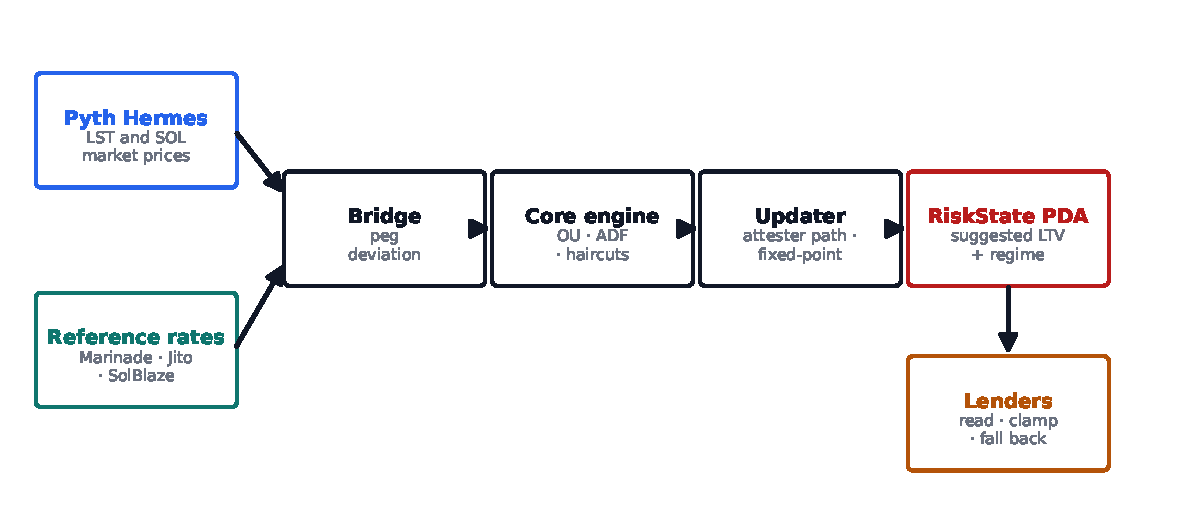
\includegraphics[width=0.95\linewidth]{system_architecture.pdf}
\caption{\label{fig:system-architecture}PegShield data plane. Pyth market feeds
and protocol reference rates are normalized by the bridge into the peg-deviation
series of Eq.~\eqref{eq:peg-deviation}, calibrated by the off-chain engine, encoded
into a fixed-point payload by the updater or attester path, and committed to a
\texttt{RiskState} PDA consumed by lending protocols.}
\end{figure*}

\subsection{Risk-State Commitment}

The on-chain artifact is an Anchor account \texttt{RiskState}
\cite{anchor_framework}, a program-derived address \cite{solana_pda} seeded by the
market identifier:
\begin{widetext}
\begin{equation}
\operatorname{PDA}_a
= \operatorname{findProgramAddress}\bigl([\texttt{"risk"},\, \operatorname{bytes}(a)],\; \texttt{program\_id}\bigr).
\end{equation}
\end{widetext}
The implemented fields are listed in Table~\ref{tab:riskstate}. Storing the state
per market under a deterministic seed gives consumers a single, stable address to
read regardless of how the write path is governed.

\begin{table*}[t]
\caption{\label{tab:riskstate}\texttt{RiskState} account fields. Real-valued
parameters are stored in fixed point at scale $10^6$.}
\centering
\begin{tabular}{lll}
\toprule
Field & Type & Meaning \\
\midrule
\texttt{lst\_id} & \texttt{String} & Market identifier, max 16 bytes. \\
\texttt{theta\_scaled} & \texttt{i64} & OU mean-reversion speed $\theta \times 10^6$. \\
\texttt{sigma\_scaled} & \texttt{i64} & OU volatility $\sigma \times 10^6$. \\
\texttt{z\_score\_scaled} & \texttt{i64} & Current z-score $z \times 10^6$. \\
\texttt{regime\_flag} & \texttt{u8} & $0=$ normal, $1=$ critical. \\
\texttt{suggested\_ltv\_bps} & \texttt{u16} & Suggested LTV in basis points. \\
\texttt{slot} & \texttt{u64} & Slot of last accepted update. \\
\texttt{timestamp} & \texttt{i64} & Unix time of last accepted update. \\
\texttt{authority} & \texttt{Pubkey} & Writer in single-attester mode. \\
\texttt{last\_updater} & \texttt{Pubkey} & Most recent submitting signer. \\
\texttt{update\_mode} & \texttt{u8} & $0=$ single-attester, $1=$ multi-attester. \\
\texttt{attester\_registry} & \texttt{Pubkey} & Registry PDA in multi-attester mode. \\
\bottomrule
\end{tabular}
\end{table*}

The oracle program performs no floating-point computation on-chain. Its role is to
validate account identity, signer authority, update mode, numeric bounds, timing,
and threshold-attester state transitions. In single-attester mode the update
instruction requires the stored \texttt{authority} as signer, rejects accounts in
multi-attester mode, checks that the supplied identifier matches the PDA state,
enforces $\theta_{\mathrm{scaled}}\geq 0$, $\sigma_{\mathrm{scaled}}>0$, and
$0\leq \mathrm{LTV}_{\bps}\leq 10000$, and rate-limits updates to at least 30
seconds apart. This keeps the trusted on-chain logic small and auditable while the
stochastic estimation remains off-chain.

\section{Statistical Model and Solvency Index}
\label{sec:model}

\subsection{Ornstein--Uhlenbeck Calibration}

The engine fits an OU model \cite{ou} to the peg-deviation series of
Eq.~\eqref{eq:peg-deviation}. In continuous time,
\begin{equation}
\dd X_t = \theta(\mu-X_t)\dd t+\sigma\dd W_t,
\label{eq:ou}
\end{equation}
where $\theta>0$ is the mean-reversion speed, $\mu$ the local equilibrium
deviation, $\sigma>0$ the instantaneous volatility, and $W_t$ a standard Brownian
motion. We estimate the discretized AR(1) regression on the increments
\cite{hamilton1994,vasicek1977},
\begin{equation}
\Delta X_i = \alpha+\beta X_{i-1}+\varepsilon_i,
\label{eq:ar1}
\end{equation}
with sampling interval $\Delta t$ in days, and map the estimates back to OU
parameters via
\begin{equation}
\hat{\theta}=-\frac{\hat{\beta}}{\Delta t},\qquad
\hat{\mu}=\frac{\hat{\alpha}}{-\hat{\beta}},\qquad
\hat{\sigma}=\frac{\operatorname{sd}(\hat{\varepsilon})}{\sqrt{\Delta t}}.
\label{eq:ou-map}
\end{equation}
Positive lower bounds ($\theta,\sigma\geq 10^{-6}$) prevent degenerate zero
estimates. The baseline parameters $(\bar{\theta}_t,\bar{\sigma}_t)$ are medians of
$\hat\theta$ and $\hat\sigma$ over rolling windows when sufficient history exists,
and the current-window estimate otherwise. Intuitively, a healthy peg reverts
quickly with low volatility (large $\theta$, small $\sigma$); a stressed peg
reverts slowly or not at all (small $\theta$) with elevated $\sigma$.

\subsection{Regime Detection}

The current standardized deviation over the rolling window $[t-n,t]$ is
\begin{equation}
z_t=\frac{X_t-\bar{X}_{[t-n,t]}}{s_{[t-n,t]}}.
\label{eq:zscore}
\end{equation}
We additionally apply the Augmented Dickey--Fuller test
\cite{adf,said_dickey1984} to the rolling window, yielding a unit-root $p$-value
$p_{\mathrm{ADF},t}$. The critical-regime indicator is the \emph{conjunction}
\begin{equation}
C_t=
\one\!\left\{|z_t|>2.5\right\}\cdot
\one\!\left\{p_{\mathrm{ADF},t}\geq 0.05\right\}.
\label{eq:critical}
\end{equation}
That is, \texttt{CRITICAL} requires both an extreme standardized deviation
\emph{and} failure to reject the unit root (loss of stationarity). Requiring both
conditions avoids treating an ordinary large variance realization in an otherwise
mean-reverting series as a structural break, consistent with the distinction
between a transient deviation and a regime change drawn in the structural-break
literature \cite{andrews1993,bai_perron2003}.

\subsection{Liquidity and Data-Quality Risk}

LST solvency depends on more than the price path. Let $L_t$ denote effective exit
liquidity available to liquidators and arbitrageurs and let $H_t\in[0,1]$ denote a
latent stake-pool health variable capturing delegation performance, withdrawal
friction, and reference-rate reliability. Peg stability can be modeled as a
jump-diffusion extension of Eq.~\eqref{eq:ou},
\begin{equation}
\dd X_t
= \theta_t(\mu_t-X_t)\dd t+\sigma_t\dd W_t
- \kappa_L\dd N^L_t
- \kappa_H\dd N^H_t,
\label{eq:jump-model}
\end{equation}
where liquidity and health shocks arrive with state-dependent intensities
\begin{widetext}
\begin{equation}
\lambda^L_t = \lambda^L_0\exp\!\Bigl(\beta_L\bigl(1-\tfrac{L_t}{L^\star_t}\bigr)_+\Bigr),
\qquad
\lambda^H_t = \lambda^H_0\exp\!\Bigl(\beta_H(1-H_t)_+\Bigr).
\end{equation}
\end{widetext}
Equation~\eqref{eq:jump-model} is the model that motivates treating liquidity and
source degradation as first-class risk; the present implementation does not yet
ingest validator-performance telemetry as a live field. It uses the canonical
staking exchange rate as the accounting reference and converts available signals
into two bounded haircuts: a liquidity haircut $h^L_t$ computed from generic depth,
slippage, pool-imbalance, withdrawal-delay, and concentration metrics when present,
and a data-quality haircut $h^Q_t$ computed from Pyth confidence ratios,
history-source fallback, reference-rate fallback, and the absence of liquidity
metrics. Both are bounded:
\begin{equation}
h^L_t\in[0,0.30],\qquad h^Q_t\in[0,0.15].
\label{eq:haircut-bounds}
\end{equation}

\subsection{The Published LTV and the Solvency Index}

With base constants $\ell_0=0.80$, $\ell_{\min}=0.40$, and $\ell_{\max}=0.80$, the
statistical LTV is
\begin{equation}
\ell^{\mathrm{stat}}_t =
\begin{cases}
\ell_{\min}, & C_t=1,\\[2pt]
\clip\!\left(
\ell_0\,
\dfrac{\hat{\theta}_t}{\bar{\theta}_t}\,
\dfrac{\bar{\sigma}_t}{\hat{\sigma}_t},\;
\ell_{\min},\;
\ell_{\max}
\right), & C_t=0.
\end{cases}
\label{eq:stat-ltv}
\end{equation}
The multiplicative form rewards fast reversion and penalizes elevated volatility
relative to the rolling baseline; a critical regime collapses the LTV to the floor
unconditionally. The published LTV applies the haircuts and re-clips:
\begin{equation}
\ell_t =
\clip\!\left(\ell^{\mathrm{stat}}_t-h^L_t-h^Q_t,\;\ell_{\min},\;\ell_{\max}\right).
\label{eq:published-ltv}
\end{equation}
We summarize the enforced constraint by the normalized \emph{solvency index}
\begin{equation}
\Psi_t=\frac{\ell_t}{\ell_0}\in\left[\tfrac12,\,1\right],
\label{eq:psi}
\end{equation}
where $\Psi_t=1$ permits the base collateral factor and $\Psi_t=\tfrac12$ is the
configured 40\% floor. For a lending market with collateral value $V_t$ and
requested debt $B_t$, PegShield's reference credit constraint is
\begin{equation}
B_t \leq V_t\,\ell_t.
\label{eq:borrow-constraint}
\end{equation}
The protocol remains free to impose a stricter cap, fall back, pause, or apply its
own liquidation policy; PegShield supplies the time-varying upper bound, not the
final decision.

\subsection{Off-Chain to On-Chain Serialization}

The boundary between stochastic off-chain estimation and deterministic on-chain
state is a fixed-point encoding at scale $10^6$, with the suggested LTV converted
to basis points:
\begin{lstlisting}
theta_scaled      = round(theta * 1_000_000)
sigma_scaled      = round(sigma * 1_000_000)
z_score_scaled    = round(z_score * 1_000_000)
suggested_ltv_bps = round(clip(ell, 0, 1) * 10_000)
\end{lstlisting}
The on-chain program validates the bounds in Section~\ref{sec:arch} but never
recomputes the model; the integrity of the estimation is enforced socially and
economically through the attester path rather than re-executed in the runtime.

\section{Decentralized Updates: Threshold Attesters}
\label{sec:attester}

A single trusted writer is a single point of failure. The implemented
multi-attester path decentralizes the writer while preserving the consumer
interface: protocols still read the same \texttt{RiskState} PDA, and the change is
confined to how writes are authorized. The design borrows from bonded and
optimistic oracle security models \cite{uma_optimistic_oracle,breidenbach2021chainlink}:
attesters post a bond, propose and confirm updates by threshold, and can be
disputed and slashed for bad updates within a challenge window. Table~\ref{tab:attester}
lists the implemented constants and accounts.

\begin{table}[h]
\caption{\label{tab:attester}Implemented threshold-attester constants and accounts.}
\resizebox{\linewidth}{!}{%
\begin{tabular}{ll}
\toprule
Item & Implemented behavior \\
\midrule
\texttt{MAX\_ATTESTERS} & 5 fixed registry slots. \\
\texttt{MIN\_ATTESTER\_BOND} & 1 SOL minimum registration bond. \\
\texttt{PENDING\_UPDATE\_TTL} & 300 seconds. \\
\texttt{DISPUTE\_WINDOW} & 3600 seconds after finalization. \\
\texttt{RESOLUTION\_DEADLINE} & 24 hours after a dispute is filed. \\
\texttt{UNREGISTER\_COOLDOWN} & 7 days before bond withdrawal. \\
\texttt{SLASH\_PERCENT} & 50\% of the attester bond. \\
\texttt{DISPUTER\_REWARD} & 50\% of the slashed amount. \\
\texttt{AttesterRegistry} & Admin, threshold, minimum bond, slash destination, attester entries. \\
\texttt{PendingUpdate} & Round payload, proposer, expiry, confirmation bitmap, finalization metadata. \\
\texttt{DisputeRecord} & Evidence hash, disputed attester, deadline, outcome, copied parameters. \\
\bottomrule
\end{tabular}
}
\end{table}

The update cycle, illustrated in Fig.~\ref{fig:attester-cycle}, is:
\begin{enumerate}
\item \texttt{initialize\_registry(threshold, min\_bond)} creates the registry PDA
and sets admin, threshold, minimum bond, and slash destination.
\item \texttt{register\_attester(bond)} transfers lamports from the attester to the
registry PDA and records an active slot; bond withdrawal is subject to a 7-day
cooldown.
\item \texttt{enable\_multi\_attester(lst\_id)} switches a \texttt{RiskState} from
single- to multi-attester mode once the registry can satisfy its threshold.
\item \texttt{propose\_update} opens a pending round; the proposer must be active
and auto-confirms via a bitmap bit indexed by registry position.
\item \texttt{confirm\_update} requires a registered, not-yet-confirming attester
and a non-expired pending round. When the confirmation count reaches the threshold,
the risk parameters are copied into \texttt{RiskState} and the round is finalized.
\item \texttt{cancel\_expired} closes an expired unfinalized round and refunds rent
to the proposer.
\item \texttt{dispute\_update} may be filed within the dispute window against an
attester that participated in the round.
\item \texttt{resolve\_dispute} is admin-gated; on a slash, 50\% of the attester's
bond is deducted, half to the disputer and half to the configured destination.
\end{enumerate}

\begin{figure*}[t]
\centering
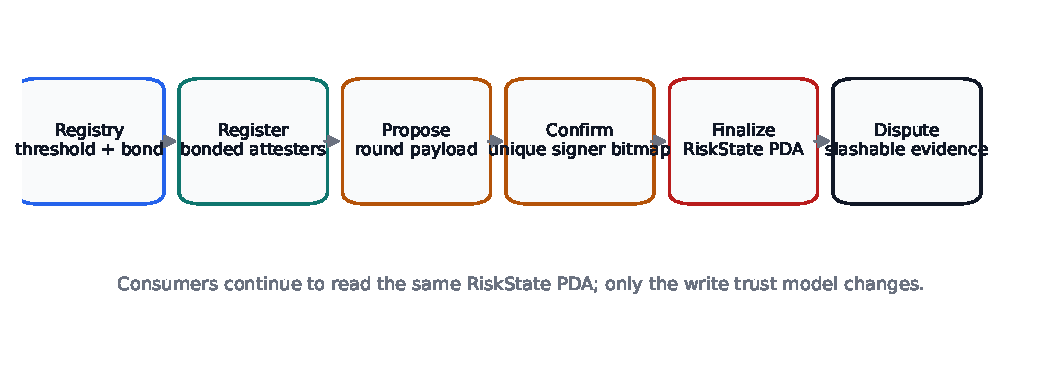
\includegraphics[width=0.98\linewidth]{attester_cycle.pdf}
\caption{\label{fig:attester-cycle}Threshold-attester lifecycle. The consumer PDA
remains stable while the write path moves from a single authority to bonded
proposal, threshold confirmation, finalization, and dispute resolution.}
\end{figure*}

The program authenticates attesters by Solana transaction-signer identity and
registry membership. It does not yet implement an on-chain Ed25519 aggregate-signature
verifier over an off-chain canonical payload; the readiness of the state machine is
therefore distinct from the operation of an independent production committee, a gap
we return to in Section~\ref{sec:discussion}.

\section{Consumer Integration}
\label{sec:consumer}

PegShield is designed to be consumed in three ways: off-chain or client-side
through a typed client library, directly inside another Anchor program by deriving
and decoding the PDA, and through a reference borrow gate that records auditable
decisions. The first two are mechanical; we describe the reference policy and the
borrow gate, which encode the intended asymmetric use of the feed.

\subsection{Reference Consumer Policy}

A conservative consumer treats staleness and critical regime as reasons to
\emph{reduce} exposure, never to increase it. The reference policy maps the
on-chain state $S_t$ to an applied LTV by
\begin{widetext}
\begin{equation}
\operatorname{safeLtv}(S_t)=
\begin{cases}
\ell_{\mathrm{fallback}}, & \operatorname{stale}(S_t),\\
\ell_{\mathrm{fallback}}, & S_t.\mathrm{regimeFlag}=1,\\
\min\!\bigl(\max(S_t.\mathrm{suggestedLtv},0),\,\ell_{\mathrm{protocolMax}}\bigr), & \text{otherwise},
\end{cases}
\label{eq:safeltv}
\end{equation}
\end{widetext}
where staleness defaults to an age beyond 600 seconds and an account whose
timestamp is zero is treated as stale. A client verifies that the account is owned
by the expected program and decodes the fixed-point layout before applying
Eq.~\eqref{eq:safeltv}; the default fallback is 40\% and example consumers cap the
maximum at a protocol-selected ceiling.

\subsection{On-Chain Borrow Gate}

The reference borrow gate is an Anchor program that reads the PegShield
\texttt{RiskState} through a cross-program account constraint, validates that the
identifiers match, and records a borrow decision with the applied LTV, oracle age,
a reason code, and an allow/reject outcome. Its decision logic is
\begin{widetext}
\begin{equation}
\ell^{\mathrm{applied}}_t =
\begin{cases}
0, & \text{policy paused},\\
\ell_{\mathrm{fallback}}, & \text{oracle stale},\\
0, & \text{critical and halt-on-critical},\\
\ell_{\mathrm{fallback}}, & \text{critical and not halt-on-critical},\\
\min\!\bigl(\ell^{\mathrm{oracle}}_t,\ell_{\mathrm{policyMax}}\bigr), & \text{otherwise},
\end{cases}
\label{eq:gate}
\end{equation}
\end{widetext}
and the borrow is permitted only when the requested debt does not exceed
$V_t\,\ell^{\mathrm{applied}}_t$. The gate demonstrates that the published
constraint is enforceable inside a borrow transaction without any governance
action, which is the property that distinguishes PegShield from an off-chain
parameter recommendation (Table~\ref{tab:positioning}).

\section{Evaluation}
\label{sec:eval}

\subsection{Methodology}

We evaluate the policy surface in two complementary ways. First, a
\emph{historical replay} drives the engine with reconstructed market data from the
June 2022 stETH/ETH discount and compares the resulting dynamic LTV against a fixed
80\% collateral factor on a modeled collateral position. Second, a
\emph{scenario suite} drives the engine with synthetic stress paths to exercise the
policy under shapes of stress that are rare in the short on-chain history of Solana
LSTs. We report what each method establishes and, equally, what it does not.

The historical replay uses archived ETH daily closes and published stETH discount
anchors interpolated into a daily window from 18 May to 30 June 2022, with a
warm-up of 20 points preceding 24 replay rows. The collateral model is 100 units of
a stETH-like asset; ``shortfall'' is the scenario-scale dollar amount by which a
position's debt exceeds its collateral value under each policy. The dynamic
borrower is modeled as listening to the most conservative LTV PegShield reaches
during the event, which isolates the value of \emph{timing}---tightening before the
worst drawdown---rather than modeling liquidator microstructure.

\subsection{Historical stETH/ETH Replay}

Table~\ref{tab:replay} and Figs.~\ref{fig:steth-ltv}--\ref{fig:shortfall} summarize
the replay. PegShield emits its first critical signal on 2022-06-09 at a peg
deviation of $-3.40\%$, four days before the fixed-80\% baseline first exhibits
modeled shortfall on 2022-06-13. Over the window, the fixed-80\% policy reaches a
peak modeled shortfall of \$51{,}946.38 on the 100-unit position, while the
PegShield policy---already at its 40\% floor---records \$0.00 modeled shortfall, a
peak LTV cut of 40 percentage points ($\Psi_t$ falling from $1$ to $\tfrac12$).

\begin{table*}[t]
\caption{\label{tab:replay}Historical stETH/ETH replay (selected rows). Shortfall
is scenario-scale dollars on a modeled 100-unit position. The \emph{PegShield LTV}
column reports the running minimum (most conservative LTV reached to date) that the
modeled borrower follows, which is why it remains at the $40\%$ floor on
\texttt{NORMAL} rows after a prior \texttt{CRITICAL} signal; consequently the
PegShield shortfall is an \emph{upper bound} on the timing benefit rather than a
per-slot causal measurement (see Section~\ref{sec:discussion}).}
\centering
\begin{tabular}{lrrlrrrr}
\toprule
Date & Peg dev. & $z$ & Regime & PegShield LTV$^{\dagger}$ & Static LTV & PS shortfall & Static shortfall \\
\midrule
2022-06-07 & $-2.40\%$ & $-1.62$ & NORMAL   & 50.1\% & 80.0\% & \$0.00 & \$0.00 \\
2022-06-09 & $-3.40\%$ & $-2.96$ & CRITICAL & 40.0\% & 80.0\% & \$0.00 & \$0.00 \\
2022-06-13 & $-4.00\%$ & $-1.88$ & NORMAL   & 40.0\% & 80.0\% & \$0.00 & \$7{,}525.44 \\
2022-06-16 & $-7.00\%$ & $-2.97$ & CRITICAL & 40.0\% & 80.0\% & \$0.00 & \$30{,}182.25 \\
2022-06-19 & $-6.27\%$ & $-1.91$ & NORMAL   & 40.0\% & 80.0\% & \$0.00 & \$51{,}946.38 \\
2022-06-30 & $-4.00\%$ & $-0.19$ & NORMAL   & 40.0\% & 80.0\% & \$0.00 & \$39{,}763.20 \\
\bottomrule
\end{tabular}
\\[2pt]
{\footnotesize $^{\dagger}$Running minimum adopted by the modeled borrower, not the
instantaneous per-slot LTV; the per-slot policy returns to a higher LTV on
\texttt{NORMAL} rows.}
\end{table*}

\begin{figure}[h]
\centering
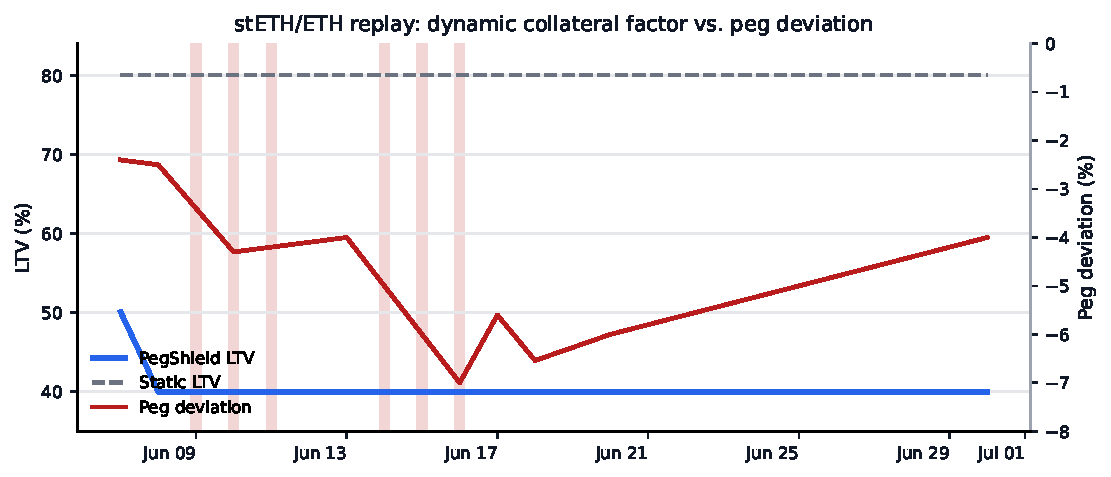
\includegraphics[width=0.92\linewidth]{steth_ltv_peg.pdf}
\caption{\label{fig:steth-ltv}Historical stETH/ETH replay. The dynamic LTV falls
from the static 80\% baseline to the 40\% floor as peg deviation deteriorates,
i.e.\ $\Psi_t$ moves from $1$ to $\tfrac12$.}
\end{figure}

\begin{figure}[h]
\centering
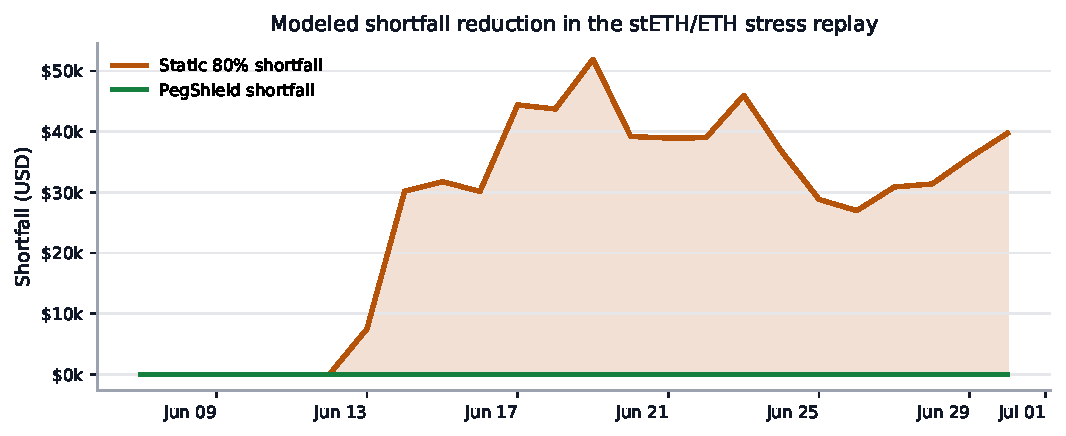
\includegraphics[width=0.92\linewidth]{shortfall_reduction.pdf}
\caption{\label{fig:shortfall}Modeled shortfall for the same replay. The static
80\% policy develops positive shortfall as the discount widens; the PegShield
policy has already tightened to the floor.}
\end{figure}

The takeaway is timing: a feed-speed risk constraint emits its first protective
signal (the \texttt{CRITICAL} flag on 2022-06-09) before a static collateral factor
produces visible shortfall in the replay. We treat the \$0.00 PegShield shortfall as
an \emph{upper bound} on the achievable timing benefit, not a causal guarantee, and
we discuss the look-ahead nature of the modeled borrower in
Section~\ref{sec:discussion}.

\subsection{Synthetic Stress Suite}

To check the policy beyond a single event, we drive the engine with eight
synthetic stress paths spanning complementary failure modes, and we report the
same shortfall and regime metrics as for the historical replay
(Table~\ref{tab:scenarios}). The paths are constructed on the modeled 100-unit
position used throughout, and the metrics are computed by the same engine and
policy code that produces the on-chain state.

\begin{table*}[t]
\caption{\label{tab:scenarios}Stress-suite results (one historical replay and eight
synthetic paths) on the modeled 100-unit position. ``Static shortfall'' and
``PegShield shortfall'' are peak modeled dollars under the fixed-80\% baseline and
under PegShield; ``Critical rows'' counts rows flagged \texttt{CRITICAL} by
Eq.~\eqref{eq:critical}; ``Recovered'' indicates the regime returned to monitoring
rather than remaining latched at the floor. Synthetic paths are regression tests
for the policy surface, not empirical market measurements.}
\centering
\footnotesize
\begin{tabular}{@{}llrrrc@{}}
\toprule
Scenario & Risk focus & Static shortfall & PegShield shortfall & Critical rows & Recovered \\
\midrule
\texttt{steth\_june\_2022} & Historical collateral impairment & \$51{,}946 & \$0 & 6 & Yes \\
\texttt{reflexive\_bank\_run} & Reflexive deleveraging & \$165 & \$0 & 15 & Yes \\
\texttt{liquidity\_vacuum} & Liquidity vacuum & \$32 & \$0 & 17 & Yes \\
\texttt{slow\_grind\_depeg} & Slow creeping impairment & \$0 & \$0 & 13 & Yes \\
\texttt{flash\_crash\_repricing} & Flash crash / snapback & \$0 & \$0 & 11 & Yes \\
\texttt{svb\_weekend\_bank\_run} & Weekend redemption panic & \$0 & \$0 & 16 & Yes \\
\texttt{stablecoin\_redemption\_spiral} & Reflexive liquidation spiral & \$0 & \$0 & 22 & Yes \\
\texttt{restaking\_bridge\_contagion} & Cross-venue contagion & \$0 & \$0 & 20 & Yes \\
\texttt{false\_positive\_wick} & Noise resilience & \$0 & \$0 & 4 & Yes \\
\bottomrule
\end{tabular}
\end{table*}

Two properties are worth separating. First, \emph{loss prevention}: in three of the
nine scenarios the fixed-80\% baseline incurs modeled shortfall while PegShield does
not, for an aggregate modeled loss prevented of \$52{,}143 on the idealized
position---a figure dominated by the historical replay, with the two synthetic
deleveraging paths contributing small amounts. Second, and more informative for the
synthetic suite, is \emph{regime behavior}: in the remaining six scenarios neither
policy breaches the idealized 80\% position, yet PegShield still tightens during the
stress window (reflected in the critical-row counts) and then recovers to
monitoring rather than latching at the floor. The \texttt{false\_positive\_wick}
path is the control: a single large but stationary deviation produces only four
critical rows and a prompt recovery, because the conjunction in
Eq.~\eqref{eq:critical} requires loss of stationarity, not merely a large $z$.
Sustained, non-stationary deterioration---the \texttt{stablecoin\_redemption\_spiral}
and \texttt{restaking\_bridge\_contagion} paths---instead produces long critical
runs (22 and 20 rows). This is the intended precision/recall tradeoff: the detector
reacts to structural breaks while tolerating transient noise. We caution that the
synthetic shortfall figures are small precisely because the idealized 100-unit
position is conservative; they characterize the \emph{policy surface}, not realized
losses, liquidator behavior, or venue-specific liquidity.

\section{Security and Manipulation Analysis}
\label{sec:security}

\subsection{Manipulation Surface}

By normalizing the market LST/SOL ratio with a protocol reference rate
(Eq.~\eqref{eq:peg-deviation}), PegShield is less sensitive to ordinary USD-price
drift than a naive LST/USD spread. To move the signal, an adversary must influence
the relative LST/SOL market price, the Pyth feed, or the canonical reference-rate
source. The implemented defenses are:
\begin{itemize}
\item on-chain writers cannot submit $\theta<0$, $\sigma\leq 0$, or an LTV outside
$[0,10000]$ basis points;
\item single-attester writes require the stored authority and are rate-limited to
one update per 30 seconds;
\item multi-attester writes require active bonded registry members and threshold
confirmation before finalization, with a dispute-and-slash window;
\item source degradation is represented as a data-quality haircut rather than
silently ignored, and missing liquidity metrics are penalized;
\item consumers verify account ownership, decode the layout, and check freshness
and regime before use, with an asymmetric policy that lowers LTV or halts borrowing
on stale, missing, or critical data.
\end{itemize}
These mechanisms reduce, but do not eliminate, manipulation risk. PegShield
inherits a dependence on Pyth honesty and timeliness
\cite{pyth2022whitepaper,eskandari2021sok} and on reference-rate integrity; it does
not currently cross-check Pyth against a secondary oracle, and it does not recompute
the OU/ADF logic on-chain. The Mango Markets incident \cite{rekt_mango_2022} is a
reminder that a manipulated input to collateral logic is sufficient for loss; the
peg normalization and the asymmetric consumer policy are mitigations, not
guarantees.

\subsection{Composability}

Because the primary output is a single PDA per market rather than a bespoke
integration, a protocol can consume PegShield off-chain through a client, directly
in an Anchor program by deriving $[\texttt{"risk"},\,\texttt{lst\_id}]$ under the
program ID, or through the reference borrow-gate pattern. The design deliberately
does not require a lender to surrender final risk authority: protocols retain their
own maximum LTVs, fallbacks, pauses, and critical-regime behavior, and PegShield
supplies the time-varying upper bound of Eq.~\eqref{eq:borrow-constraint}.

\section{Discussion, Limitations, and Threats to Validity}
\label{sec:discussion}

\paragraph{Deployment status.}
The system is pre-production. The program is deployed only to Solana devnet, the
code is unaudited and upgrade-mutable, and an independent production attester
committee is not yet operating. These are deliberate limitations of a research
prototype, not claims about a live mainnet service.

\paragraph{Threats to the evaluation's validity.}
The historical replay is a reconstruction, not a record of PegShield operating in
2022: ETH closes are archived and stETH discount points are published anchors
interpolated into the window, so the exact daily path is approximate, and we have
not tested whether the timing lead survives an alternative but equally defensible
reconstruction. The shortfall figures are scenario-scale dollars on a single modeled
100-unit position, not market-wide losses. Most importantly, the modeled borrower is
\emph{non-causal}: it follows the running minimum of the LTV reached during the
event rather than the per-slot LTV the policy would have published online. This is
visible in Table~\ref{tab:replay}, where the \emph{PegShield LTV} column stays at
the floor on \texttt{NORMAL} rows that follow a prior \texttt{CRITICAL} signal,
whereas the per-slot functional (Eq.~\eqref{eq:stat-ltv}) only forces the floor when
$C_t=1$. The \$0.00 PegShield shortfall is therefore an \emph{upper bound} on the
timing benefit, not a measured causal property; a causal online policy is the
correct primary metric and is left to future work. The replay also does not model
liquidation auction latency, keeper competition, gas, venue-specific liquidity, or
borrower behavior after a margin call---all factors the liquidation literature shows
are decisive in practice
\cite{qin2021empirical,perez2021knifeedge,warmuz2022toxic}. The synthetic scenarios
are regression tests, not empirical measurements. We therefore claim that the model
\emph{signals} earlier than a static baseline in the replay, and we do \emph{not}
claim zero market-wide bad debt, production-grade liquidator performance, or
calibration validity across all LSTs.

\paragraph{Statistical-method limitations.}
Two properties of the estimator warrant caution. First, the Augmented Dickey--Fuller
test in Eq.~\eqref{eq:critical} runs on rolling windows of roughly twenty
observations, a regime in which the unit-root test has low power and unreliable
size; the ``failure to reject stationarity'' half of the critical conjunction is
thus statistically weak at this window length, and in practice the z-score component
carries most of the detection. A full power analysis and a sensitivity study over
window length and ADF lag selection are needed before the joint rule can be claimed
to outperform a z-score-only detector. Second, the OU mapping in
Eq.~\eqref{eq:ou-map} is well defined only for a mean-reverting fit
($\hat{\beta}<0$); when a window is non-stationary or trending ($\hat{\beta}\geq 0$),
$\hat{\theta}$ is clamped at its positive floor and $\hat{\mu}$ becomes ill
conditioned. This is precisely the distressed regime the system targets, so we treat
a non-mean-reverting fit as itself a distress indicator rather than a reliable
parameter estimate; making that fallback explicit and analyzing it is future work.

\paragraph{Construct and external validity.}
The LTV functional (Eq.~\eqref{eq:stat-ltv}) and the regime thresholds
(Eq.~\eqref{eq:critical}) embed constants---the $0.80$ base factor, the $0.40$
floor, the $2.5$ z-score threshold, the $0.05$ ADF level, and the haircut
bounds---that were chosen for the prototype and require per-asset, per-venue
calibration before mainnet use. Solana LSTs also have a short on-chain history
relative to the stress shapes of interest, which is why the historical anchor is an
Ethereum event; whether Solana LST pegs exhibit the same dynamics is an empirical
question this work does not settle.

\paragraph{Research agenda.}
The natural extensions follow from these limitations: a secondary price-source
cross-check; ingestion of validator and stake-pool health telemetry as a live field
feeding $H_t$ in Eq.~\eqref{eq:jump-model}; an on-chain aggregate-signature verifier
so that finalization attests to an off-chain canonical payload; formal verification
of the LTV clamp and timing invariants; immutable or multisig-controlled upgrade
authority; venue-specific liquidity-depth calibration per LST; and a
forward-looking, mainnet evaluation against realized borrow and liquidation
outcomes.

\section{Conclusion}
\label{sec:conclusion}

We presented PegShield, a Solana-native risk oracle that publishes an enforceable
collateral constraint for liquid-staking-token collateral rather than a price.
PegShield estimates peg-deviation dynamics with an Ornstein--Uhlenbeck model,
detects distress with a joint ADF/z-score regime rule, applies bounded liquidity
and data-quality haircuts, and commits a compact fixed-point risk state---a
suggested LTV and a regime flag---to a Solana PDA that a lending market can enforce
directly through a bonded, disputable attester path. We formalized the published
constraint as a normalized solvency index $\Psi_t\in[\tfrac12,1]$ and showed, in a
historical stETH/ETH replay, that a feed-speed constraint signals before a static
collateral factor exhibits modeled shortfall---reporting the loss reduction as an
upper bound on the timing benefit---while being explicit about the
prototype's pre-production status and the limits of the evidence. The contribution
is a concrete primitive that converts peg-deviation tail risk into a
machine-readable, on-chain credit boundary, reframing LST collateral management as a
continuous risk service rather than a static governance parameter.

\paragraph{Availability.}
The implementation---off-chain bridge and engine, the Anchor programs for the risk
state, attester registry, and reference borrow gate, a typed client library, an
operator interface, and the historical and synthetic stress harness---together with
the data and scripts to reproduce the evaluation in Section~\ref{sec:eval}, is
available as an open-source repository at
\url{https://github.com/Fianko-codes/PegShield}. For reproducibility, a reference
deployment of the oracle program exists on the Solana \emph{devnet} under program
identifier \texttt{DMR3rXBh8RGrKyx1mxqFVTMbyfoiuu9iYHr6s6CW23ea}, with per-asset
\texttt{RiskState} accounts derived as in Section~\ref{sec:arch}; this deployment is
for demonstration and verification only and is not a production service.

\bibliography{pegshield_refs}

\end{document}
